% Les éditions du projet EHRI

\section{Une nouvelle approche des archives numériques}

\subsection{Une initiative européenne}
L'objectif principal de l'EHRI en tant qu'infrastructure est de promouvoir la recherche sur la Shoah en facilitant l'accès aux documents d'archives, dispersés à travers le monde. Elle doit établir un plan de travail et produire régulièrement des livrables\footnote{Plan de travail et livrables pour EHRI-3~: \texttt{\href{https://www.ehri-project.eu/division-work}{https://www.ehri-project.eu/division-work}}.}.  

Lors de la deuxième phase du projet, nommée EHRI-2 et financée par le programme Horizon 2020, l'EHRI a dédié une partie de son travail au développement d'outils pour l'archivage numérique de documents concernant la Shoah. Cela a pris la forme d'un \textit{Work Package} (WP12) intitulé \enquote{\textit{New Views on Digital Archives}} (\enquote{Nouvelles perspectives sur les archives numériques}). 


\subsection{Développer les éditions numériques sur la Shoah}
L'équipe éditoriale du WP12 a défini les critères qu'elle estime essentiels à une édition numérique sur la Shoah. Parmi ces critères, nous retrouvons une interface claire, dotée d'une bonne fonctionnalité de recherche, l'intégration de leur vocabulaire contrôlé, ainsi que l'affichage des données géographiques sur une carte\footcite[p.~6]{Ehri2018}.  



\section{Les éditions en ligne EHRI}
Chaque édition est une collection\footnote{Nous emploierons les termes \enquote{édition} et \enquote{collection} indistinctement pour faire référence aux éditions en ligne EHRI.} de documents conservés dans les institutions partenaires de l'EHRI. Ce sont des éditions thématiques\footcite{EhriOnlineEditions} reflétant une période ou illustrant un phénomène.



\subsection{BeGrenzte Flucht (2018)}
La première édition publiée par l'EHRI, \enquote{\textit{BeGrenzte Flucht: Die österreichischen Flüchtlinge an der Grenze zur Tschechoslowakei im Krisenjahr 1938}} (\enquote{Fuite entravée~: les réfugié$\cdot$e$\cdot$s autrichien$\cdot$ne$\cdot$s à la frontière tchécoslovaque en 1938\footnote{Les traductions proposées pour les titres des éditions sont les nôtres.}}), a été publiée en 2018. Elle contient cent quatre documents.  

Le nazisme est une idéologie basée sur l'antisémitisme~: la population juive est considérée comme nuisible et sert de bouc-émissaire à la situation de l'Allemagne au sortir de la Première Guerre mondiale. Toutefois, le régime nazi ne semble pas souhaiter l'élimination massive et immédiate des Juifs allemands avant la guerre\footcite[p.~123]{Sallee2018}{}. Sa politique cherche avant tout à exclure et humilier les Juifs, pour les forcer à quitter le territoire\footcite[p.~22]{Bensoussan2020}. Si une grande partie de la population juive quitte l'Allemagne, le \enquote{problème} posé par la \enquote{question juive} a seulement été déplacé et se représente au fur et à mesure que le Reich étend son territoire.  

Le 12 mars 1938, l'Autriche est annexée par l'Allemagne nazie, c'est l'\enquote{\textit{Anschlu\ss{}}}, et la population juive résidant alors en Autriche est contrainte d'émigrer. La Tchécoslovaquie devient l'un des principaux refuge pour les Juif$\cdot$ve$\cdot$s autrichien$\cdot$ne$\cdot$s, mais la politique d'accueil de plus en plus restrictive de la Tchécoslovaquie conduit au blocage complet de la frontière\footnote{À propos de l'édition \enquote{\textit{BeGrenzte Flucht}} (en allemand)~: \texttt{\href{https://begrenzte-flucht.ehri-project.eu/exhibits/show/einleitung}{https://begrenzte-flucht.ehri-project.eu/exhibits/show/einleitung}}.}. L'édition \enquote{\textit{BeGrenzte Flucht}} réunit des documents d'archives principalement tchèques et autrichiens, sous la forme de rapports gouvernementaux, articles de presse et de témoignages direct de victimes et de témoins.  

\begin{figure}[h]
    \centering
    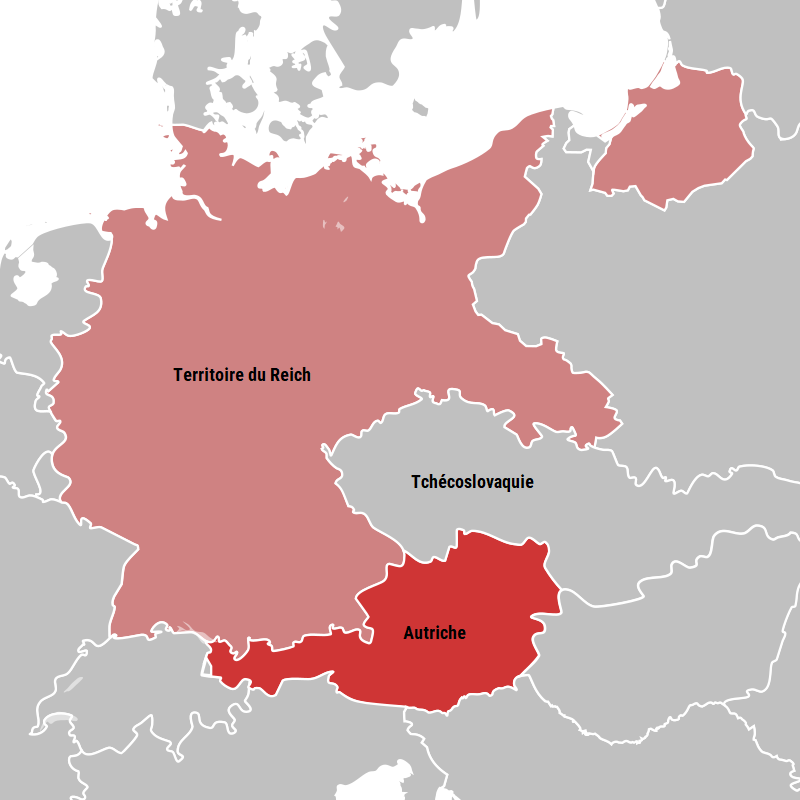
\includegraphics[width=0.8\linewidth]{2-MAIN/images/carte-anschluss.png}
    \caption{Frontières du Reich en mars 1938 (Source~: Wikipédia)}
    \label{fig:anschluss}
\end{figure}

\bigskip
\bigskip
\bigskip
\bigskip
\bigskip

\subsection{Early Holocaust Testimony (2020)}
La deuxième édition publiée par l'EHRI, \enquote{\textit{Early Holocaust Testimony}} (\enquote{Premiers témoignages de la Shoah}), a été publiée en 2020. Elle contient cent dix-neuf documents.  

Il convient tout d'abord de préciser le sens de \enquote{témoignage}. Le TLFi définit le témoignage comme une \enquote{déclaration qui confirme la véracité de ce que l'on a vu, entendu, perçu, vécu\footnote{Entrée complète sur le site du CNRTL~: \texttt{\href{https://www.cnrtl.fr/definition/temoignage}{https://www.cnrtl.fr/definition/temoignage}}}}. La collection \enquote{\textit{Early Holocaust Testimony}} se concentre sur le témoignage écrit, les témoignages oraux ayant été retranscrits. Nous reviendrons ensuite sur le terme \enquote{\textit{early}}, à propos duquel l'équipe éditoriale précise qu'il correspond à tout témoignage de la persécution de la communauté juive depuis le début du régime nazi en 1933 au procès d'Adolf Eichmann à Jérusalem en 1961\footnote{Notre propre traduction, à partir de l'introduction à l'édition (\enquote{\textit{What is an early Holocaust testimony?}})~: \texttt{\href{https://early-testimony.ehri-project.eu/exhibits/show/about/what-is-testimony}{https://early-testimony.ehri-project.eu/exhibits/show/about/what-is-testimony}}.}.


\subsection{Diplomatic Reports (2021)}
La troisième édition publiée par l'EHRI, \enquote{\textit{Diplomatic Reports}} (\enquote{Rapports diplomatiques}), a été publiée en 2021. Elle contient soixante-douze documents venant du Danemark, de l'Italie, du Japon et des États-Unis. De nouveaux rapports provenant de la Hongrie, de la Slovaquie et de la Suède devraient prochainement intégrer la collection.  

La position du$\cdot$de la diplomate est particulière~: il$\cdot$elle est amené$\cdot$e à côtoyer les politicien$\cdot$ne$\cdot$s influent$\cdot$e$\cdot$s du pays où il$\cdot$elle est stationné$\cdot$e, mais doit garder une certaine distance en tant qu'observateur$\cdot$ice. Les informations récoltées doivent être régulièrement communiquées au ministère des Affaires étrangères de leur état d'origine par le biais de rapports.

De nombreux$\cdot$ses diplomates stationné$\cdot$e$\cdot$s en Allemagne nazie ont rapidement compris que les dirigeants nazis ne se contenteraient pas des lois discriminatoires à l'encontre de la population juive. L'étude de ces rapports diplomatiques permet d'aborder la Shoah comme un événement européen auquel de nombreux pays ont activement participé, notamment par la fermeture de leurs frontières\footnote{Voir l'introduction à l'édition, rédigée par Frank Bajohr~: \texttt{\href{https://diplomatic-reports.ehri-project.eu/exhibits/show/about/introduction}{https://diplomatic-reports.ehri-project.eu/exhibits/show/about/introduction}}.}.  


\subsection{Nisko (2023)}
La quatrième édition publiée par l'EHRI, \enquote{\textit{Von Wien ins Nirgendwo: Die Nisko Deportationen 1939}} (\enquote{De Vienne à Nulle Part: les déportations vers Nisko de 1939}), a été publiée en 2023. Elle contient quarante documents.  

En avril 1938, le régime nazi ouvre son agence de l'Office central pour l'émigration juive à Vienne en Autriche\footcite[p.~30]{Bensoussan2020}. Cette agence a pour but d'accélérer l'émigration forcée des Juif$\cdot$ve$\cdot$s autrichien$\cdot$ne$\cdot$s. Au moment de l'annexion de l'Autriche en mars 1938, \enquote{plus de 200~000 personnes étaient considérées comme juives selon les critères des lois raciales de Nuremberg. Les Juifs autrichiens représentaient 40~\%{} des Juifs vivant sur tout le territoire du Grand Reich\footcite[p.~137]{Safrian2007}}. L'agence de Vienne a été libre de \enquote{tester un certain nombre de mesures extrémistes contre les Juifs\footcite[p.~132]{Safrian2007}}, autonome de l'agence principale située à Berlin.  

Le \enquote{Plan Nisko} débute en octobre 1939, un mois seulement après l'invasion de la Pologne. L'idée des dirigeants nazis est de relocaliser la population juive à Lublin et Nisko en Pologne, dans ce qu'ils appellent une \enquote{réserve juive\footcite[p.~34]{Bensoussan2020}}.  

Jusqu'à présent, la recherche sur le \enquote{Plan Nisko} s'est concentrée sur le transport et l'instrumentalisation du train comme premier projet expérimental des futures déportations de masse. La collection \enquote{\textit{Nisko}} se concentre sur la déportation d'environ 1~600 hommes juifs de Vienne les 20 et 26 octobre 1939, en seulement deux trains. Le \enquote{Plan Nisko} est abordé sous l'angle de la vie quotidienne des déportés à travers leur correspondance. Une partie de ces déportés a assuré la construction de la \enquote{réserve juive}, certains ont été capturés et envoyés dans des camps de travail russes, tandis que d'autres encore ont été \enquote{chassés vers l'Est}. Les Nazis appelaient ce phénomène la \enquote{dispersion}.  

Le \enquote{Plan Nisko} se termine en avril 1940 et des rapatriements vers Vienne sont organisés. Toutefois, le sort de ceux qui n'ont pas été rapatriés n'a pu être que partiellement reconstitué\footnote{Voir l'introduction à l'édition \enquote{\textit{Nisko}}, rédigée par Winfried Garscha~: \texttt{\href{https://nisko-transports.ehri-project.eu/exhibits/show/einleitung/nisko-transporte-wien}{https://nisko-transports.ehri-project.eu/exhibits/show/einleitung/nisko-transporte-wien}}.}.  